\subsection{Input \& Output}
The input and output of our design are shown in Table \ref{table:inputoutput}.  The external clock will allow us to connect to arbitrary clocked external input, as long as it meets the timing requirements of our design.  The 16 bit input and output are in the Q15 format described in Section \ref{sec:q15}.  The Q15 format is an industry standard, hence we expect that these required input formats are reasonable.

\begin{table}[ht]
\centering
\begin{tabular}{l | l | c}
\hline
Input/Output & Description & Bits \\
\hline \hline
Input & Clock & 1 \\
Input & Data In & 16 \\
Output & Convolution & 16 \\
\end{tabular}
\caption{Description of input and output to the filter}
\label{table:inputoutput}
\end{table}



\subsection{Power Optimization}

% Duplicate multipliers
We will optimize power by removing duplicate mulitpliers.  These duplicate multipliers are created because the filter is symmetric, therefore an adder can be used remove an adder.  In the naive filter, shown in Figure \ref{fig:naivefilter}, the constant is multiplied against each register value.  Since the constants are symmetric, ie $C0$ is the same as $C6$, this can be optimized using the associative rule.  In Figure \ref{fig:optimizedfilter}, you can see that we have removed 3 of the multipliers.  Instead, we add the values in the registers before multiplying the constants.  This eliminates 3 large and power draining multipliers.  It also simplifies the final adder from 7 input to 4.


\begin{figure}[ht]
\centering
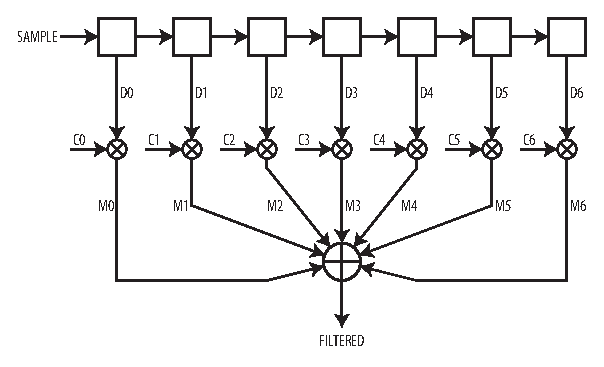
\includegraphics[width=5in]{images/filter_normal}
\caption{Naive filter implementation}
\label{fig:naivefilter}
\end{figure}

\begin{figure}[ht]
\centering
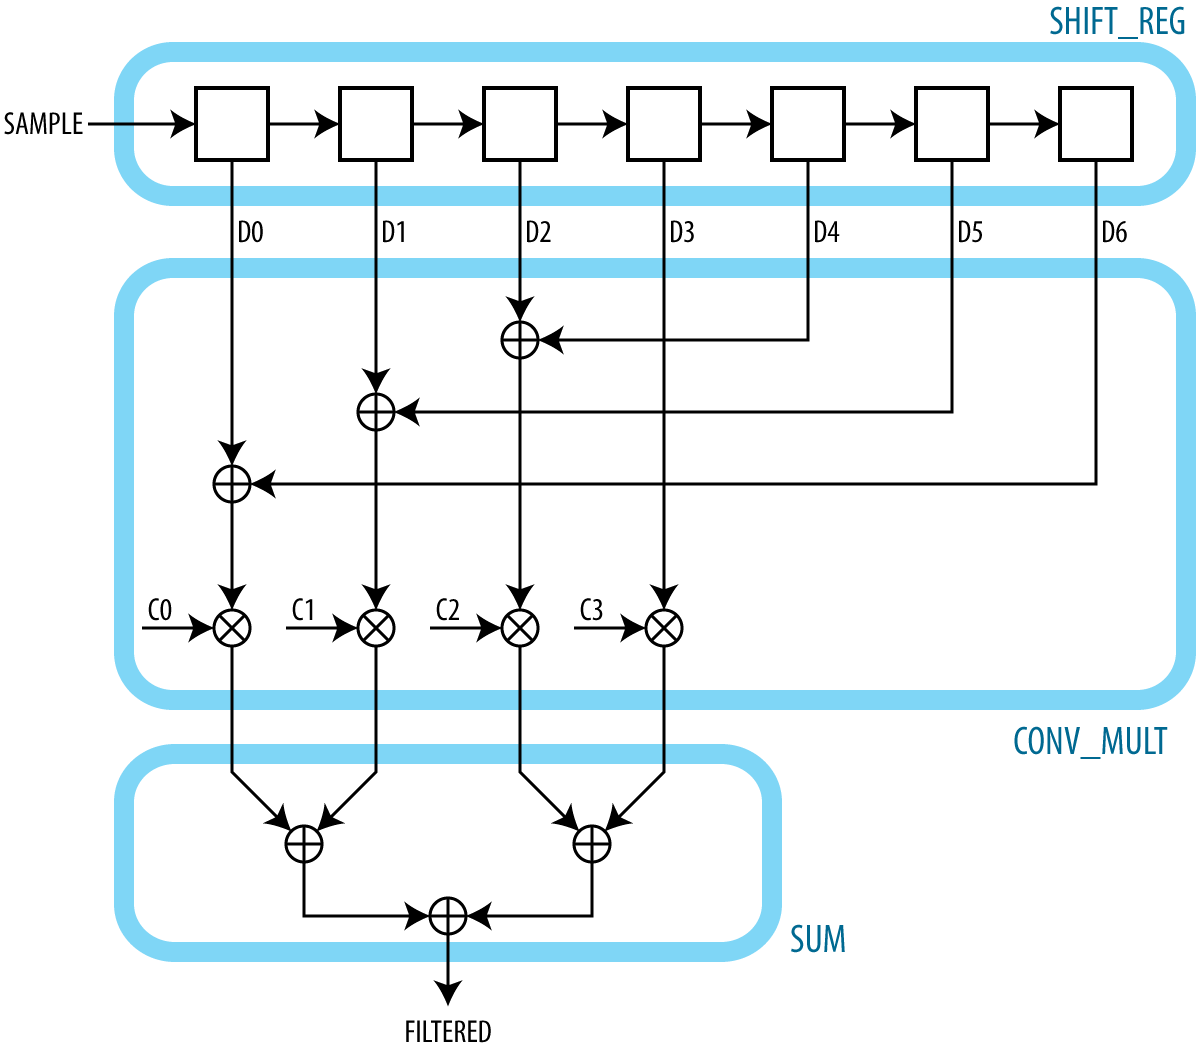
\includegraphics[width=5in]{images/filter_filtered}
\caption{Optimized filter implementation}
\label{fig:optimizedfilter}
\end{figure}

% Ripple carry adders
The adders shown at the bottom of Figure \ref{fig:optimizedfilter} are frequently changing as the final value is stabilized through the convolution hardware above.  Therefore, it is important that this hardware is optimized for power.  With reducing the number of transistors as our goal, we designed ripple-carry adders to do the final addition.  The ripple-carry adders have less hardware than the optimized version that VHDL synthesized when doing a '+'.  Also, the ripple carry adders will localize any transition to only the nodes that require it.

Compare the ripple carry to propagate/carry (PG) adders that are designed to optimize latency.  The PG adders have significantly more hardware since it has to pre-calculate propagates and carries.  



